% Generated from verified 12-epoch measurements; do not insert smoke timings.
% Provenance: ../orin_scheduling/period_sweep_protocol.txt
\begingroup
\color{blue}
\noindent\textbf{Varying the foreground inference period.}
We compare FIFO without caching and Reorder with prefetching at request periods of 105, 135, and 180\,ms.
Figure~\ref{fig:orin-period-sweep} reports the time for all 12 training epochs, excluding evaluation, using the same settings as above.
The 105\,ms results are reused from Table~\ref{tab:orin-prefetch}; we run both methods once at each of the other two periods.
Reorder with prefetching reduces training time at all three periods, by 23.97--29.85\% in these runs.
The benefit therefore persists across the tested request periods.


\begin{figure}[!t]
\color{blue}
\centering
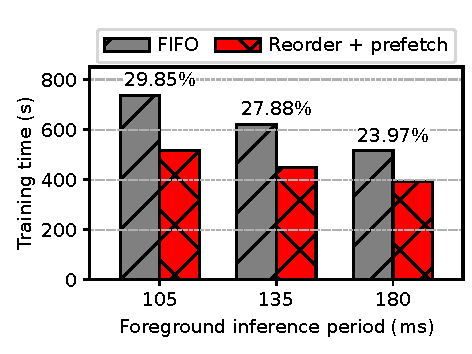
\includegraphics[width=80mm]{figures/orin_period_sweep.pdf}
\caption{Training time under different foreground inference periods. Bars show the time for 12 training epochs, excluding evaluation. Percentages show the reduction relative to FIFO without caching.}
\label{fig:orin-period-sweep}
\end{figure}
\par
\endgroup
